\documentclass{ctexart}
\textheight 23.5cm \textwidth 15.8cm
\topmargin -1.5cm \oddsidemargin 0.3cm \evensidemargin -0.3cm

\usepackage{verbatim}
\usepackage{fancyhdr}
\usepackage{float}
\usepackage{graphicx}
\usepackage{amssymb}
\usepackage{amsmath}


\pagestyle{fancy}
\CTEXsetup[format = {\Large\bfseries\it}]{section}


\begin{document}

\section*{内容简介}
	\noindent 利用四阶 Runge-Kutta 方法和各种 $\lambda$ 的值,譬如 $5$,$-5$ 或 $10$,数值求解下列初值问题:
	\begin{equation}
	\begin{cases}
		y'(x) = \lambda y + \cos x - \lambda \sin x\\
		y(0) = 0
	\end{cases}
	\end{equation}
	在区间 $[0,\,5]$ 上比较数值解和解析解。利用步长 $h = 0.01$。试问 $\lambda$ 对数值准确性有什么影响?
\section*{工作环境}
	程序所用语言: {\bf python}
	
	软件: {\bf JupyterLab}
	
	使用的包: {\bf numpy, matplotlib}

\section*{输出结果}
\begin{verbatim}
	Input lambda = -10
	Solving Equation...
	Runge-Kutta Method ended successfully
	Max Error = 1.087949252909E-08
	Reached at 1.640000000000
	
	Input lambda = -5
	...
	Max Error = 2.606221793933E-09
	Reached at 1.700000000000
	
	Input lambda = 3
	...
	Max Error = 5.811843613440E-04
	Reached at 5.000000000000
	
	Input lambda = 4
	...
	Max Error = 1.202738038629E-01
	Reached at 5.000000000000
	
	Input lambda = 5
	...
	Max Error = 2.267302864243E+01
	Reached at 5.000000000000
	
	Input lambda = 10
	...
	Max Error = 3.217088796366E+12
	Reached at 5.000000000000
	
\end{verbatim}

\begin{figure}[H]
	\centering
	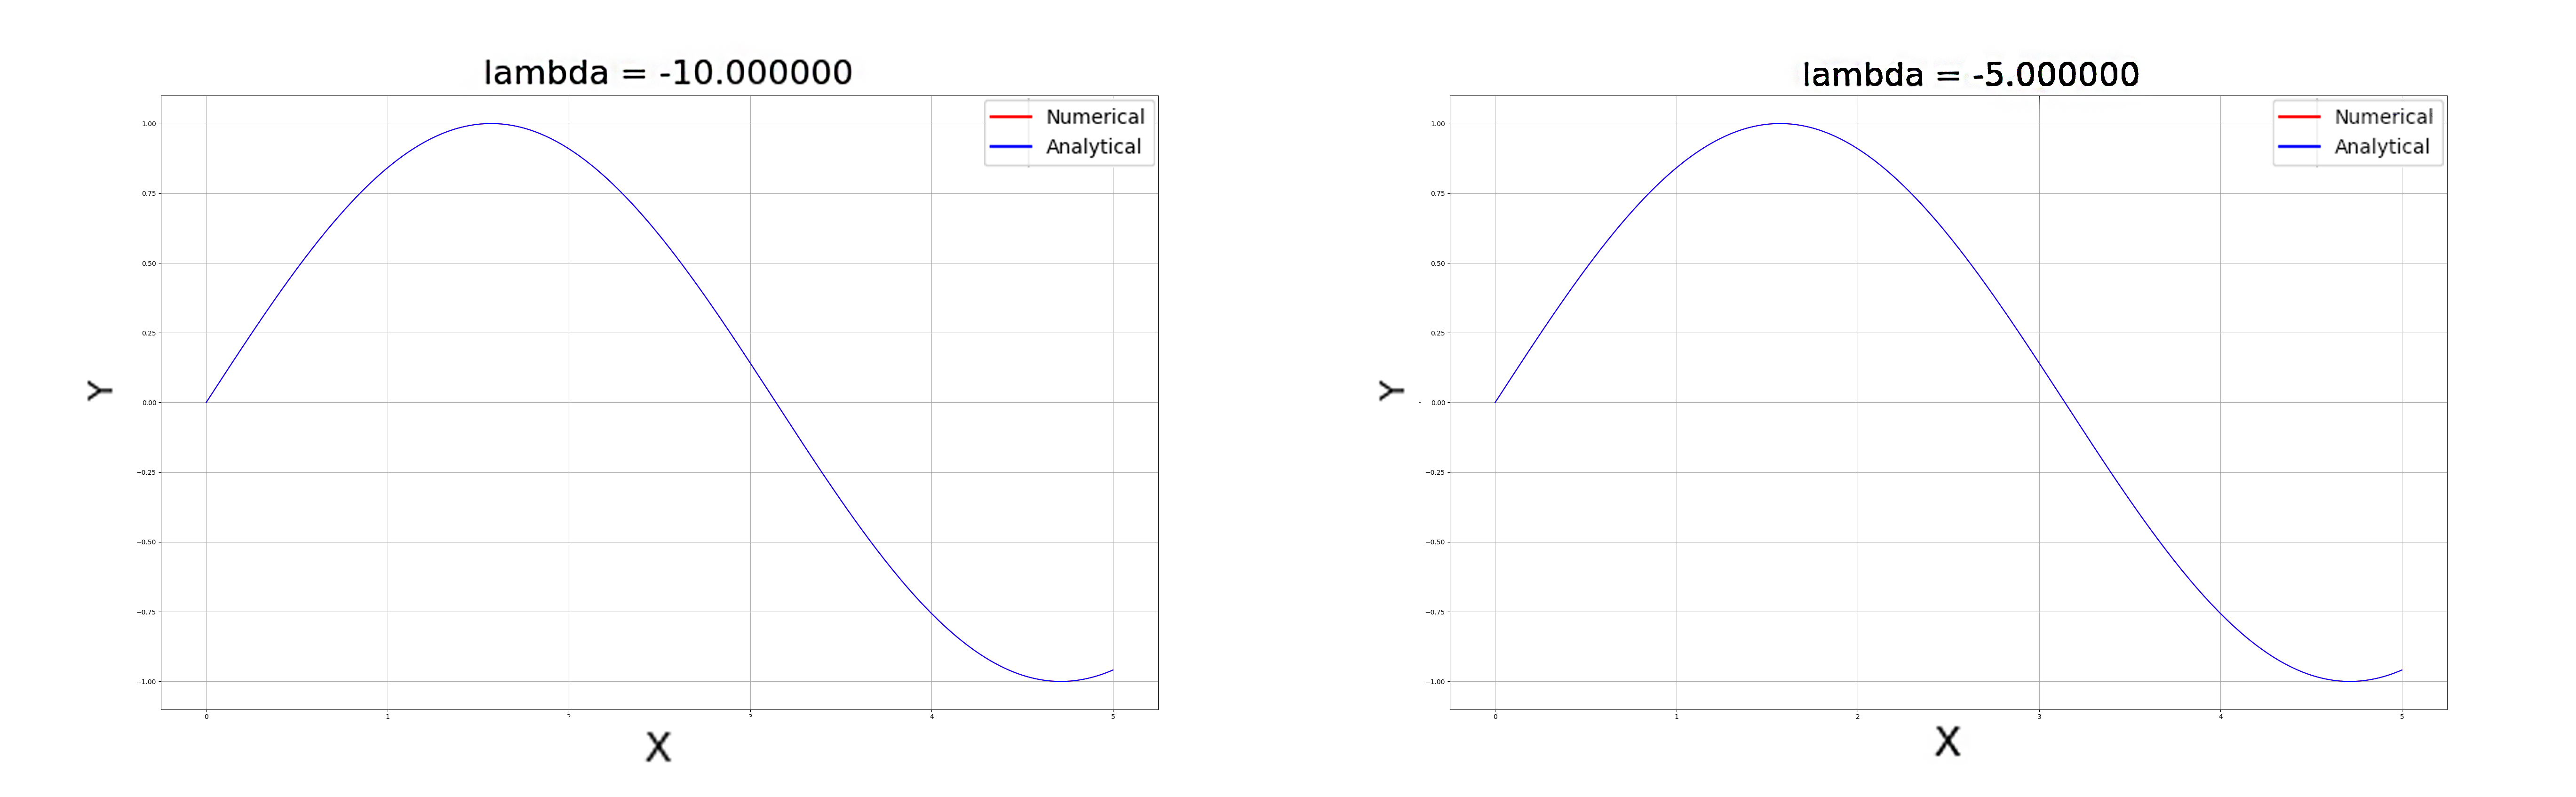
\includegraphics[width = 15cm, height = 5cm]{Figure-1.png}
	\caption{数值解与解析解比较,$\lambda = -10,\,-5$} \label{figure-1.label}
\end{figure}
\begin{figure}[H]
	\centering
	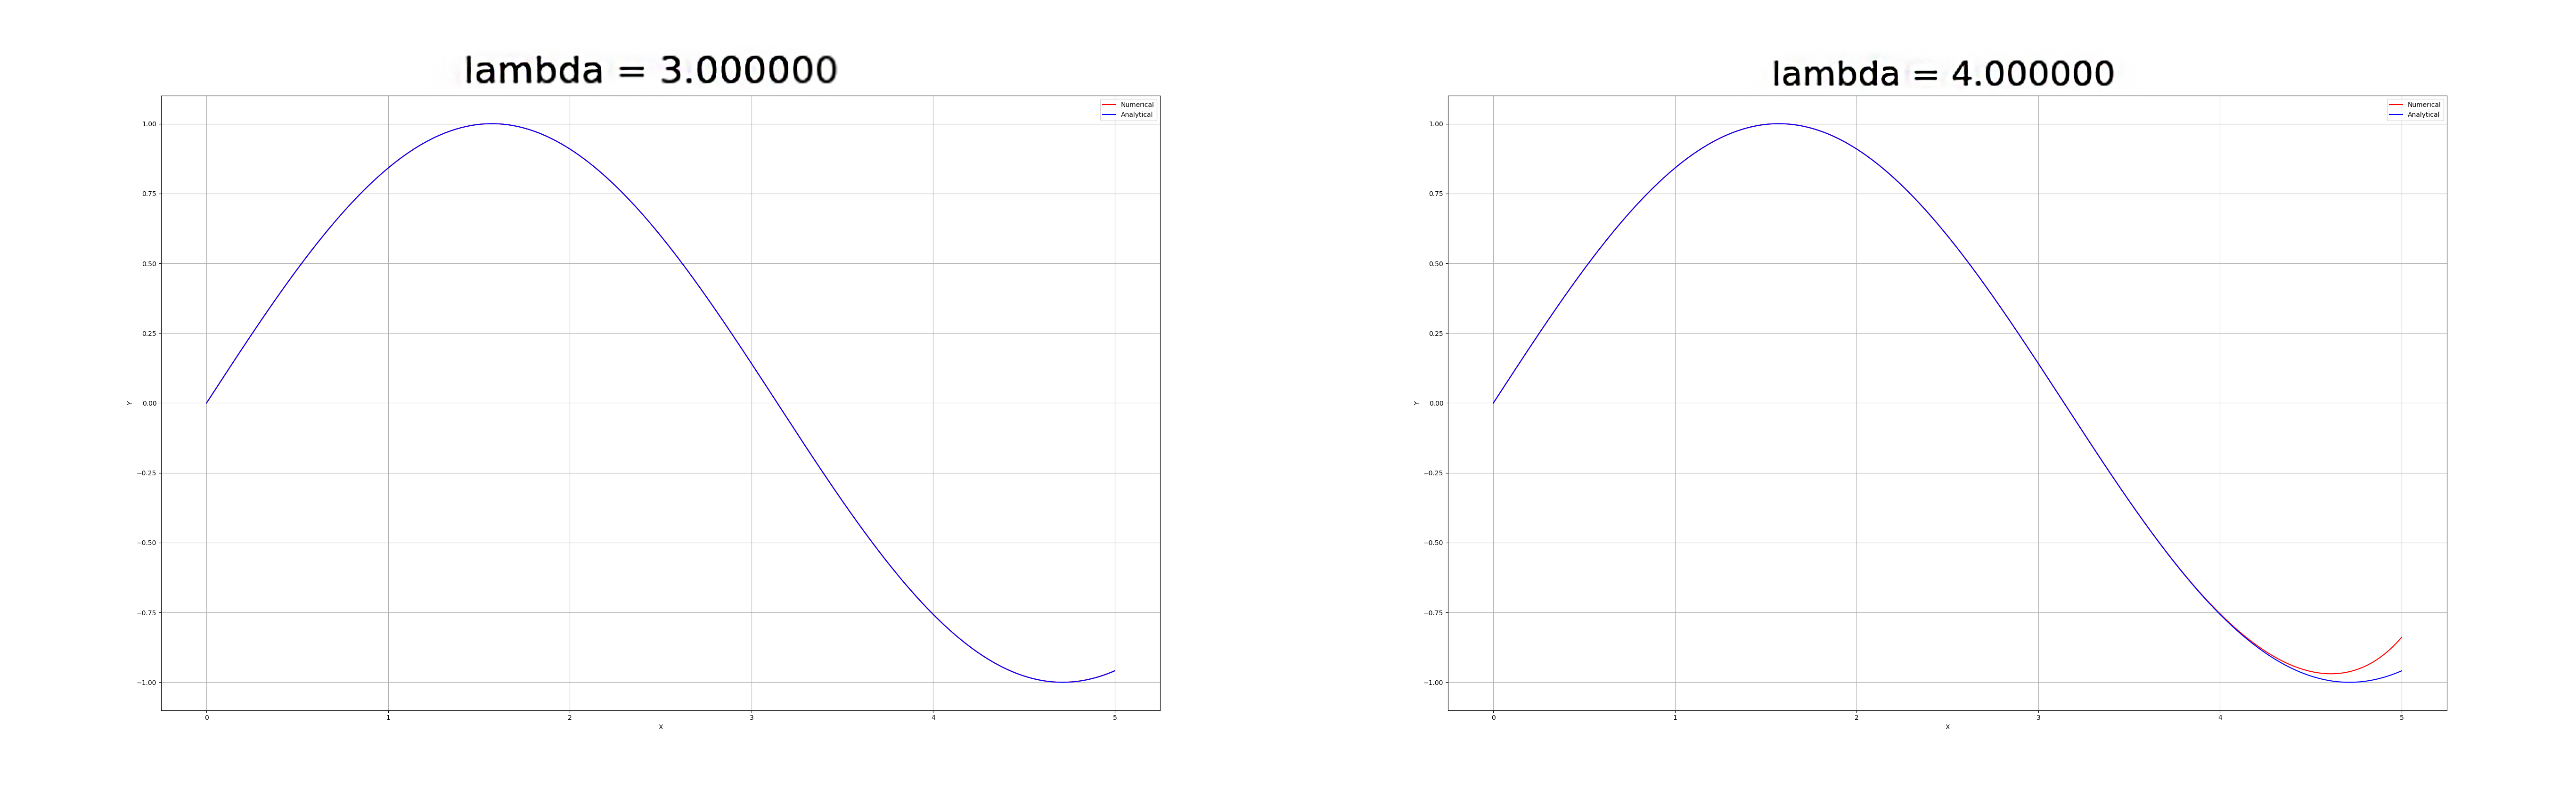
\includegraphics[width = 15cm, height = 5cm]{Figure-2.png}
	\caption{数值解与解析解比较,$\lambda = 3,\,4$} \label{figure-2.label}
\end{figure}
	\begin{figure}[H]
	\centering
	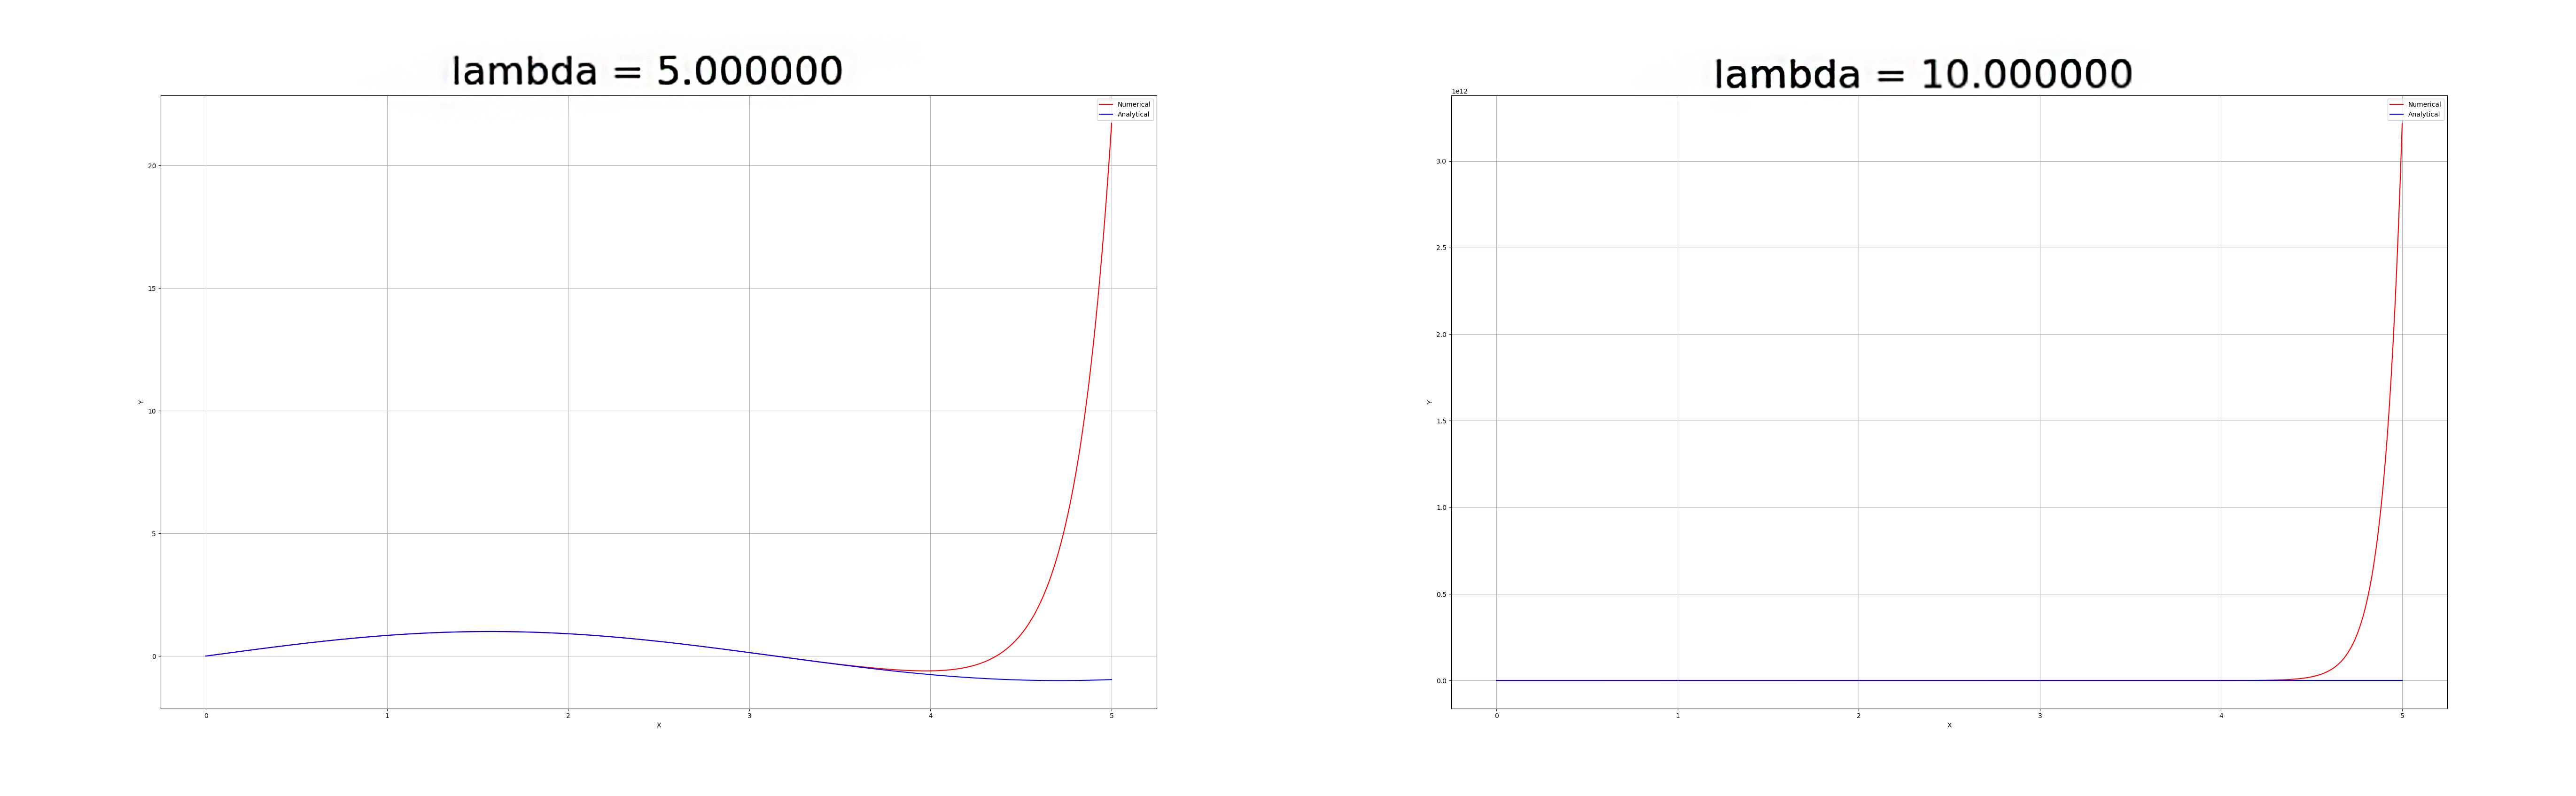
\includegraphics[width = 15cm, height = 5cm]{Figure-3.png}
	\caption{数值解与解析解比较,$\lambda = 5,\,10$} \label{figure-3.label}
\end{figure}


\section*{分析}
	容易算出该初值问题的解析解为
	\begin{equation}
		y(x) = \sin x
	\end{equation}
	图像表明 Runge-Kutta 方法在指定区间上的准确性受 $\lambda$ 影响。直观上,$\lambda$ 越大,准确性越低。且由于误差积累,越往 x轴 正向移动误差越大。下面对此现象进行简单分析。
	本实验中采用的经典的四阶 Runge-Kutta 方法为:
	\begin{equation}
		y(x + h) = y(x) + \dfrac{1}{6} (F_1 + 2 F_2 + 2 F_3 + F4)
	\end{equation}
	
	其中
	\begin{equation*}
	\left\{\begin{aligned}
		&F1 = h f(x,\,y)\\
		&F2 = h f(x + \dfrac{1}{2} h,\,y + \dfrac{1}{2} F_1)\\
		&F3 = h f(x + \dfrac{1}{2} h,\,y + \dfrac{1}{2} F_2)\\
		&F4 = h f(x + h,\,y + F_3)
	\end{aligned}\right.
	\end{equation*}
	
	考虑该步进方法中的一阶误差项:
	\begin{align*}
		y(x + h) & = y(x) + y'(x) h + O(h^2)\\
		& = y(x) + (\lambda h y + h\cos x - \lambda h \sin x) + O(h^2)
	\end{align*}
	
	因此,若令 $y_0 = y(0)$,$y_i = y(ih)$,则上式意味着
	\begin{align*}
		y_{i + 1} & = y_i + \lambda h y_i + h \cos ih - \lambda h \sin ih + O(h^2)\\
		& = (1 + \lambda h) y_i + h \cos ih - \lambda h \sin ih + O(h^2)
	\end{align*}
	
	因此有
	\begin{equation}
		y_n = \sum_{i = 0}^{n - 1} (1 + \lambda h)^{n - i} (h \cos ih - \lambda h \sin ih) + nO(h^2)
	\end{equation}
	
	故当 $\lambda \in (-\dfrac{1}{h},\,0)$ 时,
	\begin{align*}
		|y_n| & \leqslant \sum_{i = 0}^{n - 1} (1 + \lambda h)^{n - i}|1 + \lambda|h + n O(h^2)\\
		& = |1 + \lambda|(1 + \lambda h) h \dfrac{(1 + \lambda h)^n - 1}{\lambda h}+ n O(h^2)\\
		& \leqslant (1 + \lambda h) \left|\dfrac{1 + \lambda}{\lambda}\right|+ n O(h^2)
	\end{align*}
	因此 $y_n$ 有界,从而方程解的准确性得以保证。
	
	当 $\lambda \in (0,\,+\infty)$ 时,记 $\displaystyle\sum_{l = k}^r = \sum_{l = k}^r (1 + \lambda h)^{n - i} \sqrt{1 + \lambda^2}\cos(ih + \varphi)$\\
	$(a - 1) h + \varphi < \pi / 4$,$ah + \varphi > \pi / 4$;\\
	$(b - 1) h + \varphi < 0$,$bh + \varphi > 0$;\\
	$(c - 1) h + \varphi < 3 \pi / 4$,,$ah + \varphi > 3 \pi / 4$
	
	由对称性不妨认为 $\displaystyle\sum_{i = a}^{b - 1} + \displaystyle\sum_{i = b}^{c - 1} > 0$,故
	\begin{align*}
		y_n & > h \left(\sum_{i = 0}^{a - 1} + \sum_{i = c}^{n - 1}\right) + n O(h^2)\\
		& > \sqrt{\dfrac{1 + \lambda^2}{2}} \left[\sum_{i = 0}^{a - 1}(1 + \lambda h)^{n - i} - \sum_{i = c}^{n - 1}(1 + \lambda h)^{n - i} \right] + n O(h^2)\\
		& = \sqrt{\dfrac{1 + \lambda^2}{2}} (1 + \lambda h)^{n - c} \left[\sum_{i = 0}^{a - 1}(1 + \lambda h)^{c - i} - \sum_{i = c}^{n - 1}(1 + \lambda h)^{c - i}\right] + n O(h^2)
	\end{align*}
	
	因中括号内左端求和式发散而右端收敛,所以存在常数 $\Delta$ 使得对于足够大的 $n$,$\displaystyle\sum_{i = 0}^{a - 1}(1 + \lambda h)^{c - i} - \displaystyle\sum_{i = c}^{n - 1}(1 + \lambda h)^{c - i} > \Delta$,故
	\begin{equation}
		y_n > \sqrt{\dfrac{1 + \lambda^2}{2}} (1 + \lambda h)^{n - c} \Delta
	\end{equation}
	它是无界的。因此当 $\lambda > 0$,时,方程的解在足够远的距离上将不能保证准确性。图示中也体现出了这一点。
	
\section*{参考资料}
	\noindent [1] David R. Kincaid \& E. Ward Cheney. {\it Numerical Analysis: Mathematics of Scientific of Computing Third Edition}, Brooks/Cole, 2002.

\end{document}